In the study of fluid dynamic systems, the \textit{von Kármán vortex street} phenomenon stands a quintessential example of pattern formation in flows behind a bluff bodies. Characterized by alternating vortices it is not just an example of the complexity of fluid dynamics but also of great importance in various research fields influencing the design of objects in fluid- or aerodynamic systems. Simulating the Kármán vortex street plays a key role for advancements in aerodynamics, civil engineering, and environmental studies. For example the performance of a wing heavily depends on the specific flow, and therefore emergence of vortices can have an impact on the efficiency of the plane and its flight capabilities in various situations. The potential optimization of shape and coatings to achieve desired flight performances led alone in the field of aircraft engineering to a multitude of studies and research activities. Another very interesting occurrence of the phenomenon is shown in Figure \ref{fig: example vortices}, where the interplay of a mountain and wind leads to pattern formation in the clouds and forms alternating vortices. 


\begin{figure}[!htb]
        \centering
        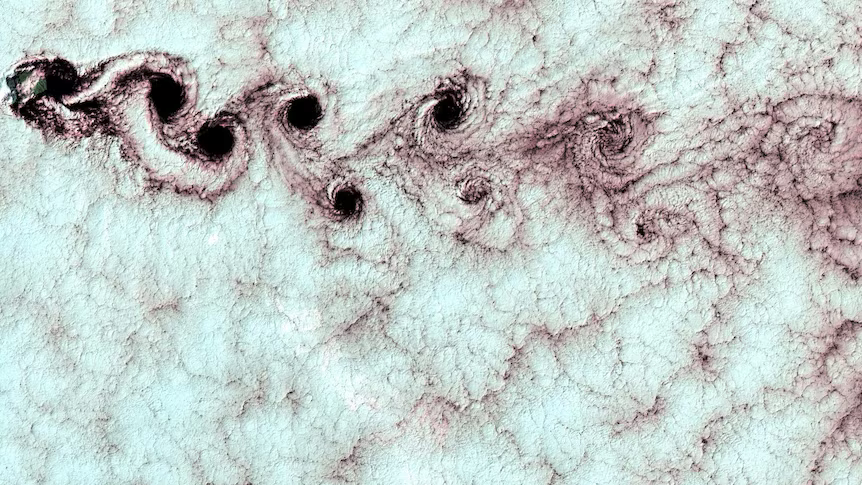
\includegraphics[width=0.6\linewidth]{0_graphics/example_atmos.png}
        \caption{View of a von Kármán vortex street in the atmosphere, showcasing the mesmerizing pattern of swirling vortices caused by airflow around a mountain.}
        \label{fig: example vortices}
\end{figure}

This project aims to numerically simulation of the phenomenon that accurately captures the dynamics of the the von Kármán vortex street behind bluff bodies in a two-dimensional flow field. By leveraging the \textit{Chorin projection method} to decouple the velocity and pressure fields and using a \textit{Semi-Langrangian} solver for the convective terms in the underlying equations, we aim to simplify the computational complexity inherent in fluid dynamics problems and to ensure stability and accuracy in the representation of vortex shedding and evolution over time.
Therefore the plan for the following report is as follows \textcolor{red}{HOW is it?}

First we introduce the underlying equations in Section \ref{}, and present and motivate the solver in Section \ref{}. In Section \ref{} we numerically simulate the system (showing that we can observe it, test different forms and compare the observationss)\\